\documentclass[12pt]{article}

\usepackage[utf8]{inputenc}
\usepackage[T1]{fontenc}  
\usepackage{hyperref}    
\usepackage{url}   
\usepackage{graphicx}
\usepackage{tabularx}
\usepackage{mathptmx}
\usepackage[romanian]{babel}
\usepackage{indentfirst}
\usepackage{subfig}

\graphicspath{ {./graphics/} }

\hypersetup{
	colorlinks=true,
	linkcolor=blue,
	filecolor=magenta,      
	urlcolor=cyan,
}
\urlstyle{same}

\newcolumntype{C}[1]{>{\centering\arraybackslash}p{#1}}


\title{\textbf{Raport final - Automatic 2D-to-3D image conversion}}

\author{
 	ECHIPĂ: E6
	\\
	 Beldiman Vladislav Student1
	\\
	Grupa 1305A
}

\begin{document}

\noindent\begin{minipage}{0.1\textwidth}
	
\includegraphics[width=1.1cm]{logo_AC.png}
\end{minipage}
\hfill
\begin{minipage}{1\textwidth}\raggedright
	Universitatea Tehnică "Gheorghe Asachi" din Iași\\
	Facultatea de Automatică și Calculatoare\\
	Prelucrarea Imaginilor - Proiect
\end{minipage}

{\let\newpage\relax\maketitle}

\maketitle
\begin{abstract}
Proiectul dat reprezintă o aplicație Windows cu interfață grafică care realizează conversia unei imagini din 2D în 3D cu interacțiune minimă în cadrul acestui proces din partea utilizatorului. Acest lucru e realizat considerând intensitatea fiecărui pixel drept valoarea înălțimii acestuia într-un câmp de înălțimi, iar pe baza acestor valori e construită o plasă poligonală cu fețe triunghiulare (Figura \ref{fig:fig1}).

Triangulația domeniului determinat de pixeli e realizată prin triangulația naivă (Figura \ref{fig:fig2}) care include toate punctele corespunzătoare pixelilor, sau prin aproximare prin înserare lacomă secvențială (Figura \ref{fig:fig3}) cu sau fără aplicarea triangulației Delaunay[1]. Înserarea lacomă va folosi drept măsură de importanță pentru fiecare punct eroarea verticală dintre valoarea câmpului și aproximarea interpolată în acel punct.

Aplicația e scrisă în limbajul de programare C++ cu interfața grafică realizată cu ajutorul setului de instrumente Qt, iar plasa poligonală e sintetizată folosind interfața pentru programarea aplicațiilor OpenGL. Ea permite vizualizarea imaginii încărcate și finale, cât și salvarea imaginii 3D în format STL.

Utilizatorul are opțiunea de a selecta algoritmul de triangulație, selecta eroarea maximă la triangulație (unde e cazul), inversara imaginea finală (răsturnarea valorilor din câmp) și selecta înălțimea dintre valoarea maximă și minimă de gri.

Am constatat faptul că utilizarea unei aproximări prin înserare lacomă fără aplicarea triangulației Delaunay de cele mai multe ori la prezența unui număr mare de triunghiuri care au un unghi cu mult mai mare decât celelalte două, care duce la un număr cu mult mai mare de puncte și triunghiuri în plasa finală, de unde rezultă și un timp mai mare de execuție, cât și, specific pentru aplicația dată, a zonelor care arată ca un burduf de acordeon unde se concentrează multe astfel de triunghiuri.

\textbf{Cuvinte cheie: \color{red} Câmp de înălțimi, Triangulație, Plasă poligonală \color{black}}
\end{abstract}

\section{Introducere}



\begin{figure}[!htb]
	\begin{minipage}{0.32\textwidth}
		\centering
		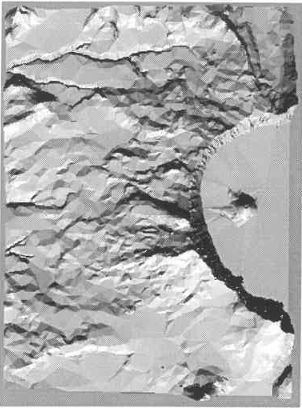
\includegraphics[width=.7\linewidth]{ExempluPlasa.png}
		\caption{Exemplu de plasă poligonală rezultantă. [1]}\label{fig:fig1}
	\end{minipage}\hfill
	\begin{minipage}{0.32\textwidth}
		\centering
		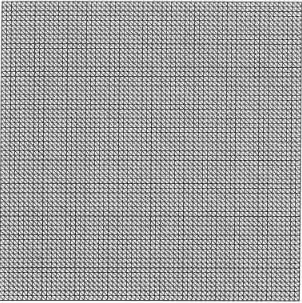
\includegraphics[width=.7\linewidth]{ExempluTriangulatieNaiva.png}
		\caption{Exemplu de triangulație naivă. [1]}\label{fig:fig2}
	\end{minipage}\hfill
	\begin{minipage}{0.32\textwidth}
		\centering
		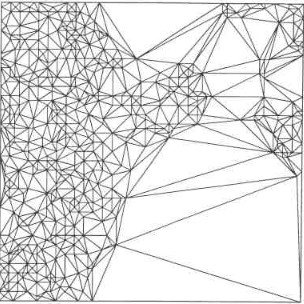
\includegraphics[width=.7\linewidth]{ExempluTriangulatieCuAproximari.png}
		\caption{Exemplu de triangulație care aproximează un câmp de înălțimi. [1]}\label{fig:fig3}
	\end{minipage}
\end{figure}

\newpage
\vspace{10cm}
\section{Metode existente}

\textbf{Git repository:} \url{https://github.com/veeyslaw/hfbm}



\section{Descrierea tehnică a soluției}




\section{Rezultate experimentale}



\section{Concluzii}



\section*{Referințe}

\medskip

[1] \href{http://reports-archive.adm.cs.cmu.edu/anon/anon/home/ftp/1995/CMU-CS-95-181.pdf} {Garland M. and Heckbert P. S. (1995) Fast Polygonal Approximation of Terrains and Height Fields. (CMU-CS-95-181)}

[2] \href{https://www.fabbers.com/tech/STL_Format#Sct_binary} {Marshall Burns. Automated Fabrication
Improving Productivity in Manufacturing.}

\end{document}